%% This is emulateapj reformatting of the AASTEX sample document
%%
\documentclass[iop]{emulateapj}

\newcommand{\vdag}{(v)^\dagger}
\newcommand{\myemail}{skywalker@galaxy.far.far.away}

%% You can insert a short comment on the title page using the command below.

\slugcomment{Not to appear in Nonlearned J., 45.}

%% If you wish, you may supply running head information, although
%% this information may be modified by the editorial offices.
%% The left head contains a list of authors,
%% usually a maximum of three (otherwise use et al.).  The right
%% head is a modified title of up to roughly 44 characters.
%% Running heads will not print in the manuscript style.

\shorttitle{Size - Star Formation}
\shortauthors{Phillips et al.}

%% This is the end of the preamble.  Indicate the beginning of the
%% paper itself with \begin{document}.

\begin{document}

%% LaTeX will automatically break titles if they run longer than
%% one line. However, you may use \\ to force a line break if
%% you desire.

\title{The Relationship Between Size and Star Formation in Active Galaxies}

%% Use \author, \affil, and the \and command to format
%% author and affiliation information.
%% Note that \email has replaced the old \authoremail command
%% from AASTeX v4.0. You can use \email to mark an email address
%% anywhere in the paper, not just in the front matter.
%% As in the title, use \\ to force line breaks.

\author{J. I. Phillips\altaffilmark{1,2,3} and Claudia Scarlata \altaffilmark{1}}
\affil{Minnesota Institute for Astrophysics, University of Minnesota,
    Minneapolis, MN 55455}

%% Notice that each of these authors has alternate affiliations, which
%% are identified by the \altaffilmark after each name.  Specify alternate
%% affiliation information with \altaffiltext, with one command per each
%% affiliation.


%% Mark off your abstract in the ``abstract'' environment. In the manuscript
%% style, abstract will output a Received/Accepted line after the
%% title and affiliation information. No date will appear since the author
%% does not have this information. The dates will be filled in by the
%% editorial office after submission.

\begin{abstract}
We examine a sample of SDSS galaxies with masses between $10^{8.5}$ and $10^{10.5}$ for signatures of radial feedback driven by bursty star formation. We measure each galaxies' offset from the mass-size relation, and plot this excess size against their $H\alpha$ emission. Below $10^{9.5}$, we see a negative correlation between galaxy size and $H\alpha$ emission. This is strong observational evidence for a ``breathing'' mode of star formation, where intense star formation in the galactic center drives radial outflows of gas and stars in a cyclic fashion. This ``breathing'' may kinematically heat the dark matter, lowering the central density of the dark matter halo and forming a cored profile. The existence of these cored profiles in dwarf galaxies stands as a significant outstanding problem with the $\Lambda CDM$ cosmological paradigm. More massive galaxies do not show the same correlations between size and star formation activity, consistent with the observations that these objects reside in cuspy dark matter halos. Additionally, we examine the radial profile of star formation in both dwarf and massive galaxies, finding star formation far more concentrated in dwarf galaxies.
\end{abstract}

%% Keywords should appear after the \end{abstract} command. The uncommented
%% example has been keyed in ApJ style. See the instructions to authors
%% for the journal to which you are submitting your paper to determine
%% what keyword punctuation is appropriate.

%% Authors who wish to have the most important objects in their paper
%% linked in the electronic edition to a data center may do so in the
%% subject header.  Objects should be in the appropriate "individual"
%% headers (e.g. quasars: individual, stars: individual, etc.) with the
%% additional provision that the total number of headers, including each
%% individual object, not exceed six.  The \objectname{} macro, and its
%% alias \object{}, is used to mark each object.  The macro takes the object
%% name as its primary argument.  This name will appear in the paper
%% and serve as the link's anchor in the electronic edition if the name
%% is recognized by the data centers.  The macro also takes an optional
%% argument in parentheses in cases where the data center identification
%% differs from what is to be printed in the paper.

%\keywords{globular clusters: general ---
%globular clusters: individual(\objectname{NGC 6397},
%\object{NGC 6624}, \objectname[M 15]{NGC 7078},
%\object[Cl 1938-341]{Terzan 8})}

%% From the front matter, we move on to the body of the paper.
%% In the first two sections, notice the use of the natbib \citep
%% and \citet commands to identify citations.  The citations are
%% tied to the reference list via symbolic KEYs. The KEY corresponds
%% to the KEY in the \bibitem in the reference list below. We have
%% chosen the first three characters of the first author's name plus
%% the last two numeral of the year of publication as our KEY for
%% each reference.

\section{Introduction}
\label{intro}

Dwarf galaxies are important laboratories that allow us to study structure formation at the smallest scales. In particular, their ratio of baryons to dark matter are extremely low, typically around 1:100. This gives rise to important differences in the structure and star formation histories of dwarf galaxies as compared to more massive galaxies, and studying these differences can shed light on important physics related to how galaxy formation is regulated by both baryons and dark matter.

Cosmological simulations based on the preferred cold dark matter model ($\Lambda$CDM) predict that galaxies form in self-similar halos of dark matter, which have density profiles described by a double power law with an inner slope of -1, termed a Navarro-Frank-White (NFW) profile \citep{NFW}. The distribution statistics and kinematics of massive galaxies is fully consistent with them living in dark matter halos with NFW profiles \citep{Wambsganss04,Springel05,BK09,Klypin11}; however, dwarf galaxy kinematics are better described by halos with a flat inner slope, typically referred to as a ``cored'' profile \citep{Moore94,McGaugh01,Marchesini02,Simon05,deblok08}. This tension between predictions made from $\Lambda CDM$ and observations is termed the ``core-cusp problem.'' A closely related problem, the ``too big to fail problem,''  notes that satellite halos (or subhalos) seen around Milky-Way-like galaxies in $\Lambda$CDM simulations are too dense to host any of the observed Milky Way dwarf satellites \citep{BK11,BK12}. Note that these two problems may indeed be two manifestations of the same problem, e.g. if halos in the real Universe have cored profiles, although that need not necessarily be the case. Recent work by \cite{GK14} demonstrated that the ``too big to fail'' problem extended beyond the Milky Way's virial radius, suggesting that the problem has more to do with how dwarf galaxies form than how environmental effects such as ram-pressure stripping or tidal interactions manifest (See, e.g., \cite{Gunn72,Larson80,Farouki81,Moore96,Balogh2000} for a discussion of these effects).

In order to resolve these problems, one of two things must be true. Either the underlying physics of $\Lambda$CDM must be modified in some way, or baryonic processes must be invoked to bridge the gap between theory and observation. Recent work has been dedicated to exploring both possibilities. On the cosmological side, both self-interacting dark matter and warm dark matter can serve to suppress structure formation and lower the central densities of dark matter halos \citep{Lovell14,Elbert14}. With respect to baryonic matter, supernova feedback has long been known to deposit energy into the interstellar medium (ISM), driving galactic winds \citep{Larson74,Dekel86}. More recently, this feedback has been posited as a mechanism by which energy may be injected into dark matter particles, kinematically warming them. Several authors have argued that if star formation proceeds stochastically in dwarf galaxies, energy will be injected with enough efficiency to create cores in the centers of dark matter halos \citep{Governato10,Governato12,PG12}. Observational studies have demonstrated that, for dwarf galaxies in particular, the star formation rate as measured by $H\alpha$ has more scatter than the star formation rate as measured by FUV emission \citep{Sullivan00,Boselli09,Shivaei15,Guo16,Sparre17}. This is consistent with a picture where star formation in dwarfs is stochastic; however, radial transport driven by this stochastic star formation remains unobserved.

One clue to resolving this dilemma may lie in how dwarf galaxies' old stars are distributed. While exceptions abound, massive galaxies generally have concentrations of old stars in the center, and younger stars in the outskirts. Dwarf galaxies, on the other hand, typically show the inverse; young stars in the center and old stars on the outskirts \citep{Hidalgo09,Hidalgo13}. Several studies have argued that these radial age gradients arise from in situ formation; old stars in the external region were born there at early times and remained there \citep{Stinson09,Schroyen13}. However, recent simulations have raise the possibility that stars in dwarf galaxies experience significant radial transport; young stars are born in galactic interiors, then at some point in their lifetimes they move to larger radii, possibly driven by feedback \citep{EB17}. Distinguishing between these two possibilities could shed light on the physics behind dwarf galaxy formation.

A unified model of galaxy formation that solves these problems was first put forward by \cite{Governato10}, where the authors show that feedback driven outflows can produce galaxies in simulations with realistically cored profiles. Further studies \citep{Governato12,EB17} refined the theory, specifying that feedback regulates dwarf galaxy star formation in a stochastic manner and powers radial transport, but an observational smoking gun for this model remains elusive. 

In this study, we use observations of both dwarf galaxies and massive galaxies to investigate the observational predictions of a model of dwarf galaxy formation whereby stochastic star formation in the center of the galaxy powers radial transport of both baryonic and dark matter. Specifically, our study will focus on the structure of star forming galaxies, and how that structure is dependent on the vigor with which the galaxy is forming stars. [Description of sections]. Throughout the paper we use h=0.7 in appropriate calculations, [other relevant details]. 

\section{Data and observations}
\label{sec:obs}

The data used in this study comes from the Sloan Digital Sky Survey \citep[SDSS,][]{SDSS}, making use of the NYU and MPA-JHU value-added galactic catalogs \citep{Kauffmann03,Brinchmann04,blanton05vagc}. To select our scientific sample, we first select all galaxies with stellar masses between $10^{8.5}$ and $10^{10.5} M_{\odot}$, where the masses are obtained by fitting spectra to synthetic spectra generated by \cite{BC03}. We require galaxies in our scientific sample to be actively star forming, so we impose a minimum $H\alpha$ equivalent width of $2 \rm \AA$ and require that the galaxies we select reside in the purely star forming region of the BPT diagram. We admit to the scientific sample only galaxies within a mass-dependent completeness redshift, estimated by dividing the sample into four mass bins of width 0.5 dex and plotting a histogram of the redshift of galaxies in each bin. The peak of the histogram was taken to be the approximate completeness limit for the scientific sample.

We also put together a sample that would be used to calibrate the fiber corrections. This sample was selected in exactly the same way as the scientific sample, except the completeness requirement was relaxed; galaxies were permitted into the calibration sample if they were within two times the completeness limit of the scientific sample. In \ref{sec:fibercor}, we describe how this calibration sample is used.

\subsection{Fiber corrections}
\label{sec:fibercor}
SDSS spectroscopy is based on light being channeled into fibers $3"$ in diameter. Because most of our galaxies are larger than 3", we must correct measured values for contributions lying outside the fiber. Typical methods for fiber correction require assuming that the inner regions of the galaxy are suitably similar to the outer regions; however we wish to refrain from making this assumption. We will later compare our fiber correction results to those following the methodology of e.g. \cite{Brinchmann04} and \cite{Salim07}.

Our correction begins by defining a parameter $\Psi$ that corresponds to the fraction of a galaxy's area on the sky that lies within the fiber. For galaxies smaller than 3", $\Psi = 1$. For larger galaxies, $\Psi = \frac{\pi R^2}{A_z}$, where R is the circularized radius of the galaxy measured in kpc (taken to be R90 so as to account for nearly all light from the galaxy) and $A_z$ is the area of a circle of diameter 3" at the redshift of the galaxy under consideration. If we are correcting some parameter $\Theta$, e.g. star formation rate, we assume that the correction will take the form $$\Theta_{total} = \Theta_{fiber} \times \Psi^{-\alpha}$$ where $\alpha$ is an power law that we derive empirically according to the following procedure.

In calculating $\alpha$, our goal is to match the measurement made on the science sample to a suitably similar comparison sample made at slightly higher redshift. This comparison set is selected to be at higher redshift so that galaxies are smaller, but not high enough that evolutionary effects must be accounted for. At this higher redshift we identify all objects that have measured diameters less than 3", but which would have diameters greater than 3" were they at the angular diameter distance of the scientific sample. Correspondingly, in the scientific sample we identify all objects that have measured diameters greater than 3", but would have diameters less than 3" at the angular diameter distance of the comparison set. These subsamples will be referred to as the high-z and low-z "calibration set." Since the low-z calibration set members are larger than the fiber, the quantity we measure is $\Theta_{fiber}$. The high-z calibration set, being selected to fall entirely within the fiber, probes $\Theta_{total}$. From here, we apply the correction given by Equation (1) to the low-z calibration set, such that the median $\Theta_{total}$ matches the median corrected $\Theta_{fiber}$. 

As a check, we applied the same aperture corrections to the full comparison sample, from which the high-z calibration set was drawn. In Figure \ref{fig:check}, we plot the uncorrected and corrected $H\alpha$ equivalent width in the scientific sample alongside the corrected $H\alpha$ equivalent width from the high-z comparison sample. We see good agreement in the corrected results at the different redshifts, suggesting that the correction made was appropriate and not biased by redshift or by the size cuts made to select the calibration sets.



%%%%%%%%%%%%%%%%%%%%%%%%%%%%%%%%%%%%%%%%%%%%%%%%%%%%%%%%%%%%%%
\begin{figure*}
	\centering
	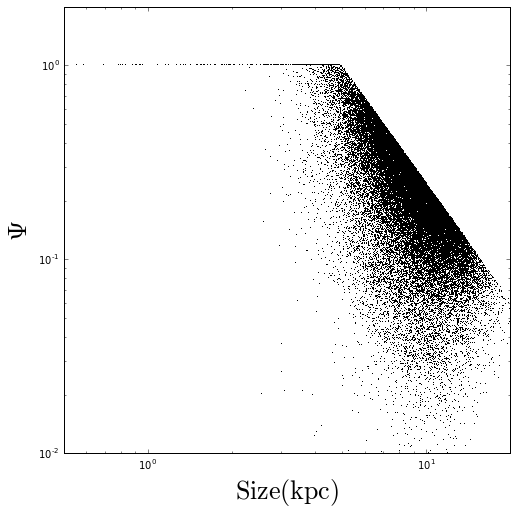
\includegraphics[width=1 \columnwidth]{geometry_10_0.png}
	\caption{Geometric parameter $\Psi$ plotted vs. physical size for galaxies in the $10^{10} - 10^{10.5} M_{\odot}$ mass bin. $\Psi$ measures the fraction of the galaxy that falls within the SDSS fiber. The selection effect arises due to the cut in redshift space.}
     \label{fig:geo}

\end{figure*}
%%%%%%%%%%%%%%%%%%%%%%%%%%%%%%%%%%%%%%%%%%%%%%%%%%%%%%%%%%%%%% 

%%%%%%%%%%%%%%%%%%%%%%%%%%%%%%%%%%%%%%%%%%%%%%%%%%%%%%%%%%%%%%
\begin{figure*}
	\centering
	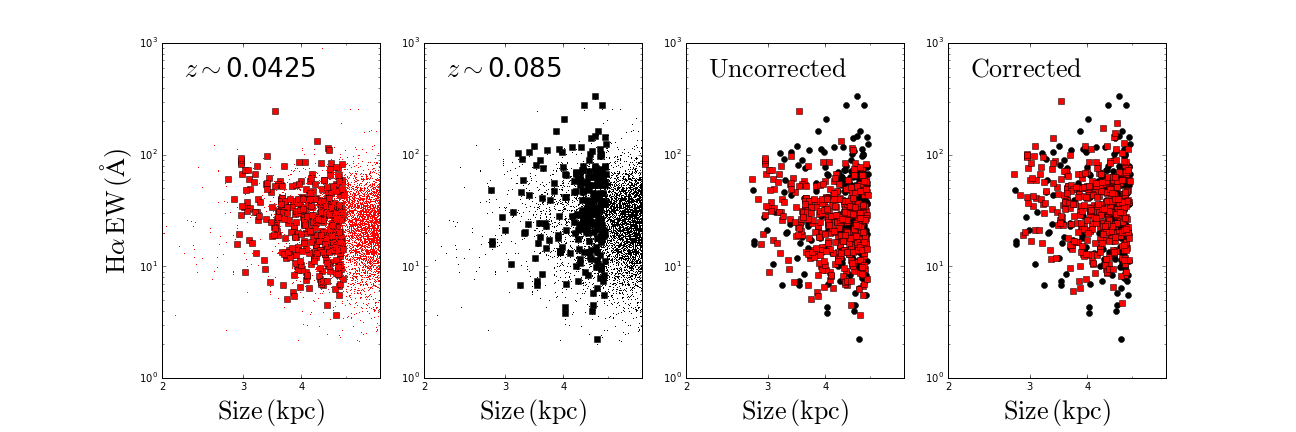
\includegraphics[width=2 \columnwidth]{steps_10_0.png}
	\caption{Figure explaining the steps involved in our aperture correction method. (1) Low z calibration set (large points) plotted alongside the scientific sample. (2) High z calibration set(large points) plotted alongside the higher z sample from which the calibration set was drawn. (3) Low z and High z calibration sets plotted together before correction. (4) Low z and High z calibration sets plotted together after correction.}
     \label{fig:steps}

\end{figure*}
%%%%%%%%%%%%%%%%%%%%%%%%%%%%%%%%%%%%%%%%%%%%%%%%%%%%%%%%%%%%%% 

%%%%%%%%%%%%%%%%%%%%%%%%%%%%%%%%%%%%%%%%%%%%%%%%%%%%%%%%%%%%%%
\begin{figure*}
	\centering
	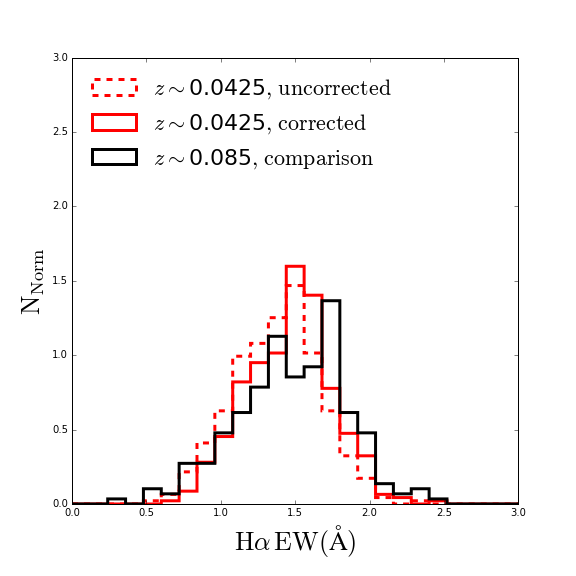
\includegraphics[width=1 \columnwidth]{hist_10_0.png}
	\caption{Histogram of $H\alpha$ equivalent widths for the uncorrected low z calibration set (dashed red line), the corrected low z calibration set (solid red line), and the high z calibration set (solid black line), which is selected to require no correction.}
     \label{fig:hist}

\end{figure*}
%%%%%%%%%%%%%%%%%%%%%%%%%%%%%%%%%%%%%%%%%%%%%%%%%%%%%%%%%%%%%% 


%%%%%%%%%%%%%%%%%%%%%%%%%%%%%%%%%%%%%%%%%%%%%%%%%%%%%%%%%%%%%%
\begin{figure*}
	\centering
	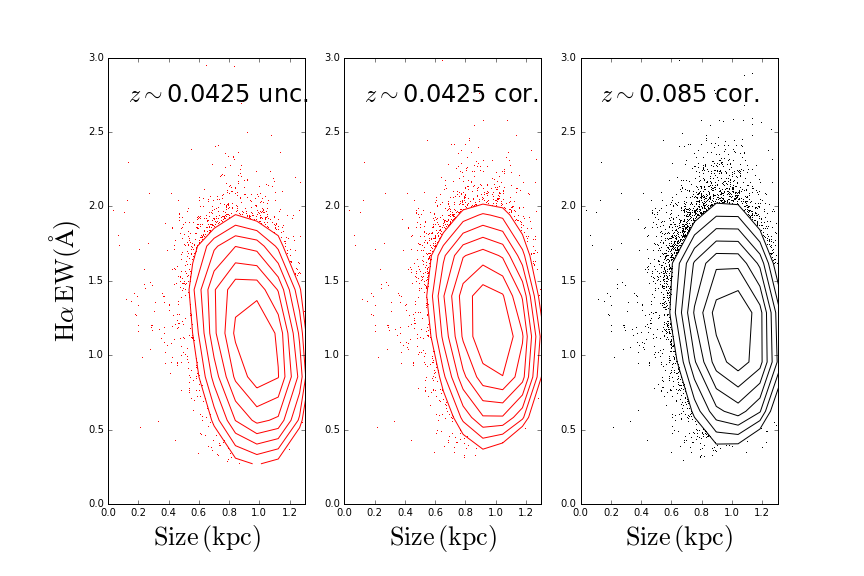
\includegraphics[width=2 \columnwidth]{all_corrected_10_0.png}
	\caption{$H\alpha$ equivalent width verusus physical size for the uncorrected scientific sample, the corrected scientific sample, against the high z sample subject to the same correction. We see good agreement in the corrected sample between low and high redshift, which is what we would expect if the we were correctly accounting for aperture effects.}
     \label{fig:check}

\end{figure*}
%%%%%%%%%%%%%%%%%%%%%%%%%%%%%%%%%%%%%%%%%%%%%%%%%%%%%%%%%%%%%% 


\section{Results}
\label{sec:results}

In Figure \ref{fig:HA_EW}, we examine the relationship between a galaxy's physical size and its rest frame $H\alpha$ equivalent width. Our sample is divided into bins of 0.5 dex in stellar mass, allowing us to examine how the relationship between size and $H\alpha$ equivalent width changes with galaxy mass.

To establish a mass-independent size metric, we fit a mass-size relation to all star-forming galaxies below redshift 0.03, then determine the expected size for each galaxy in the sample based on its stellar mass. For each galaxy, we then calculate a ``size offset" which is the logarithm of the ratio between the actual size of the galaxy in kpc and the expected size of the galaxy, also in kpc. This size offset parameter has the useful properties of being centered at or very close to zero for any given population of galaxies, and having relatively consistent scatter (about 0.4 dex) over the mass ranges we probe.

In figure \ref{fig:HA_EW}, we plot the total (i.e. aperture-corrected) $H\alpha$ equivalent width against the size offset parameters in four stellar mass bins. We find a clear change in behavior around $10^{9.5} M_{\odot}$. Above that mass, $H\alpha$ equivalent width is relatively size independent; below that mass, we see a clear anti-correlation in  $H \alpha$ equivalent width with galaxy size.

We plot $H\alpha$ luminosity against size offset in Figure \ref{fig:HA_lum} and see a broadly similar trend with stellar mass. At low mass, galaxies show no correlation between size and $H\alpha$ luminosity, whereas at high mass, $H\alpha$ luminosity tends to be higher in larger galaxies. This is consistent with the equivalent width result; highly star forming galaxies are much more likely to be compact at low masses than at high masses, and extended galaxies are more likely to have significant star formation at high masses than at low.   

In Figure \ref{fig:HA_lum}, we reproduce the lower two panels in Figure \ref{fig:HA_EW}, and estimate the duty cycle for the active phase in dwarf galaxies to be roughly 1/3 in both mass bins, based on the percentage of the population in the active and passive phases. The slope of the dividing line between active and passive was chosen to be perpendicular to the line connecting the median values. The intercept of the dividing line was (somewhat arbitrarily) chosen to be the same as the line connecting the median values, i.e. these lines intersect at a size offset of 0.0. 

%%%%%%%%%%%%%%%%%%%%%%%%%%%%%%%%%%%%%%%%%%%%%%%%%%%%%%%%%%%%%%
\begin{figure*}
	\centering
	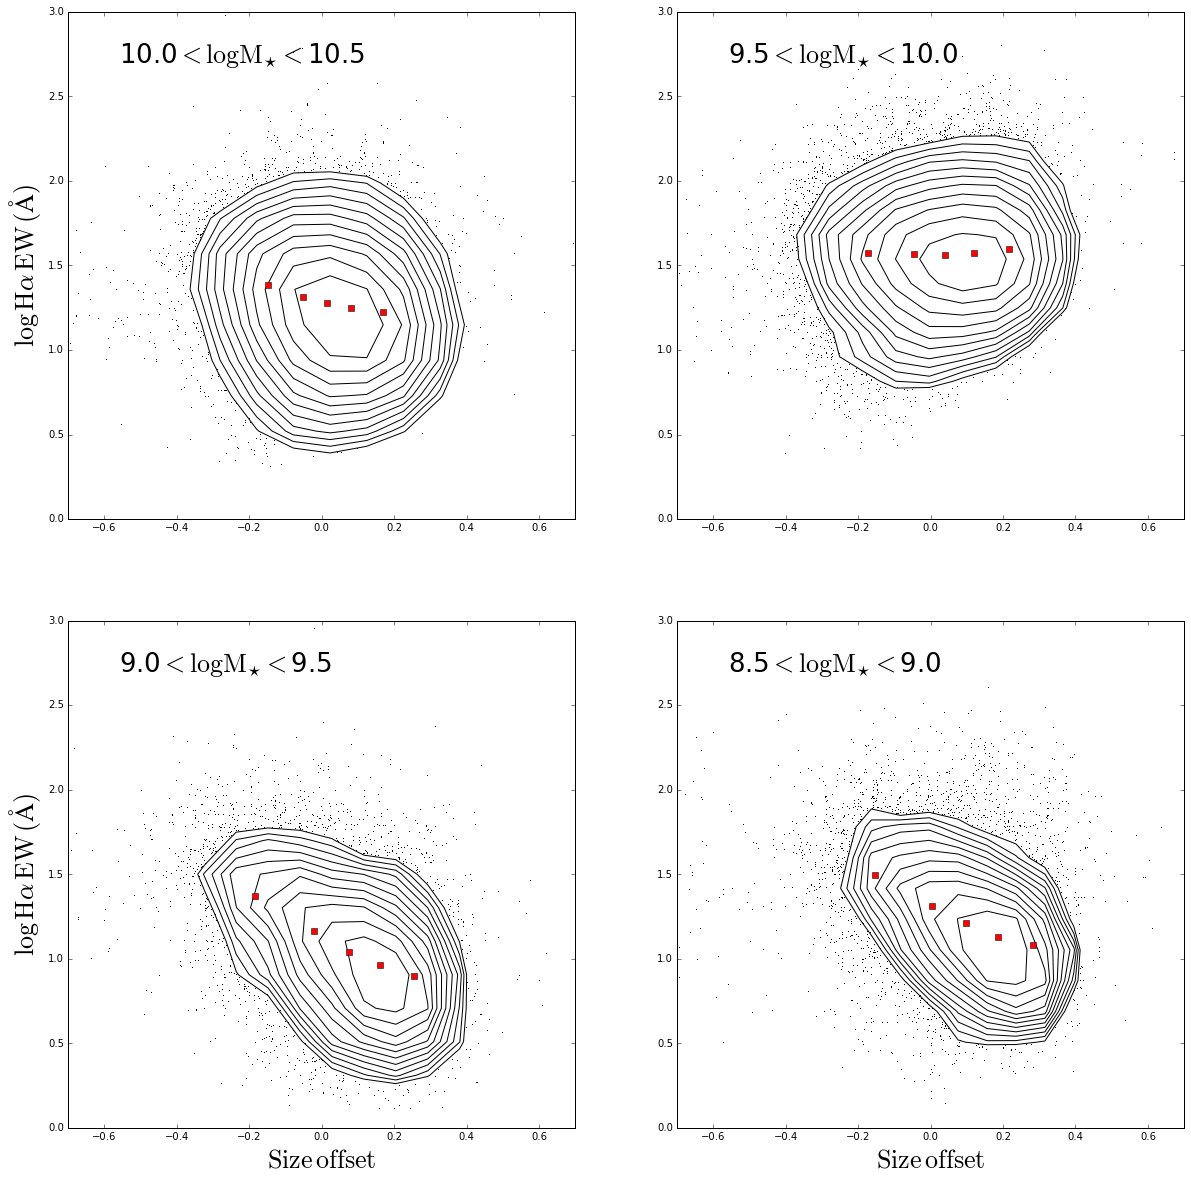
\includegraphics[width=1.5 \columnwidth]{HA_EW.png}
	\caption{Relationship between $H\alpha$ equivalent width and size offset, defined as the excess size compared to the mass-size relationship. }
     \label{fig:HA_EW}

\end{figure*}
%%%%%%%%%%%%%%%%%%%%%%%%%%%%%%%%%%%%%%%%%%%%%%%%%%%%%%%%%%%%%% 

%%%%%%%%%%%%%%%%%%%%%%%%%%%%%%%%%%%%%%%%%%%%%%%%%%%%%%%%%%%%%%
\begin{figure*}
	\centering
	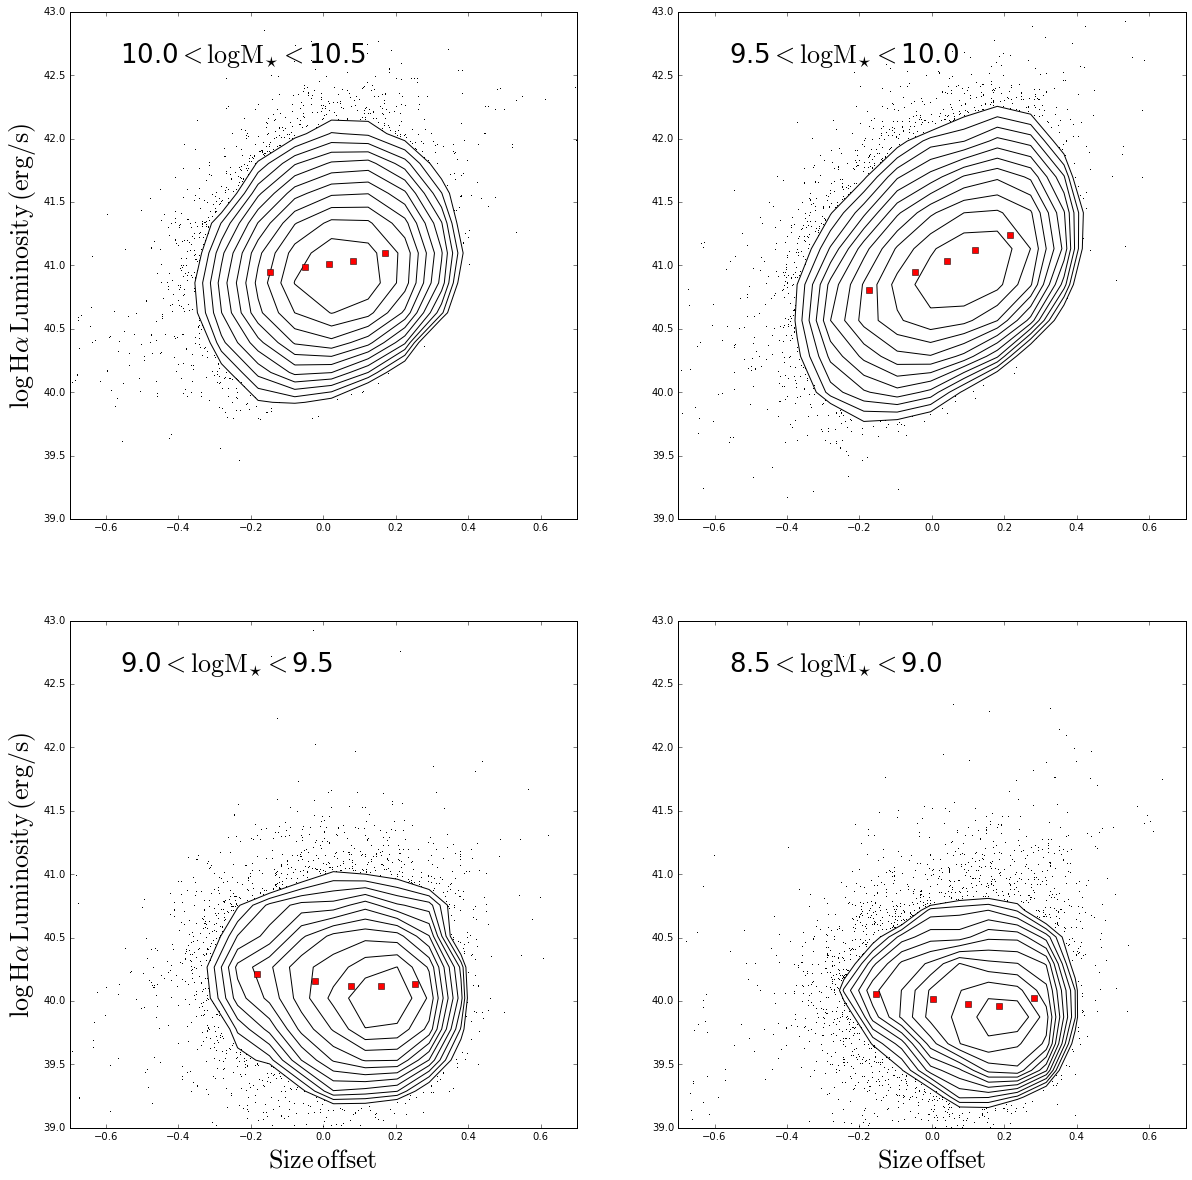
\includegraphics[width=1.5 \columnwidth]{HA_LUM.png}
	\caption{Relationship between $H\alpha$ luminosity and size offset. }
     \label{fig:HA_lum}

\end{figure*}
%%%%%%%%%%%%%%%%%%%%%%%%%%%%%%%%%%%%%%%%%%%%%%%%%%%%%%%%%%%%%% 

%%%%%%%%%%%%%%%%%%%%%%%%%%%%%%%%%%%%%%%%%%%%%%%%%%%%%%%%%%%%%%
\begin{figure*}
	\centering
	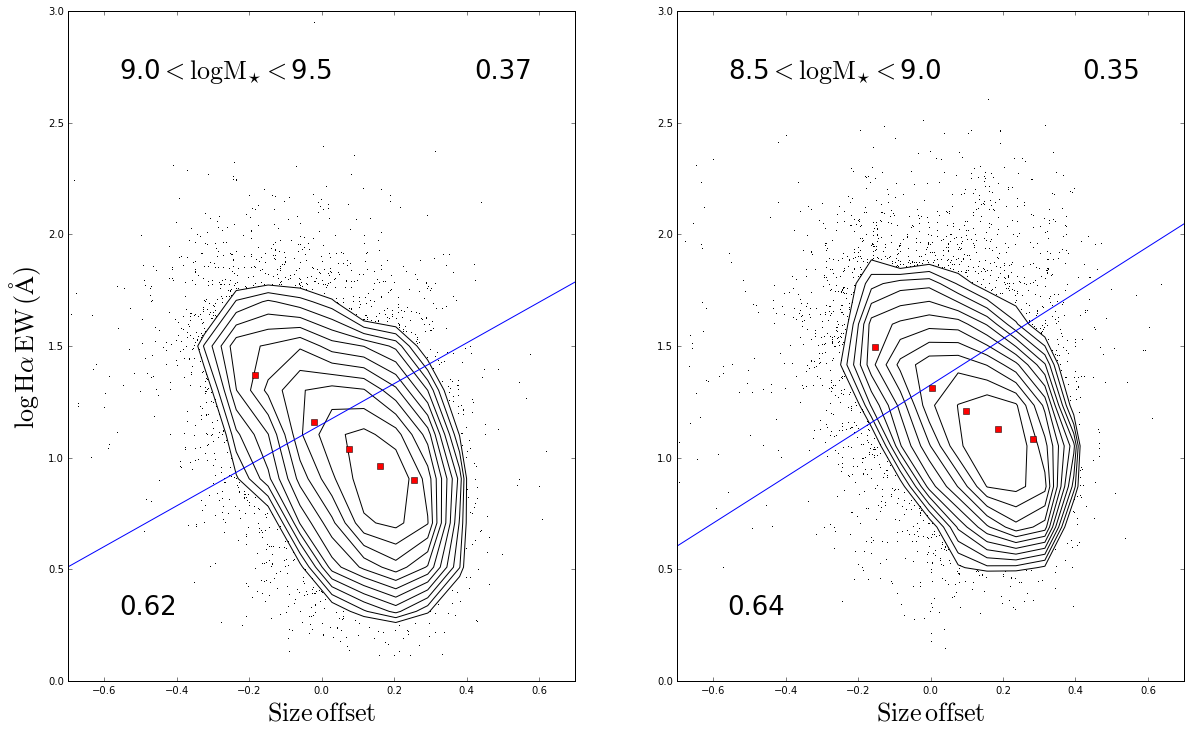
\includegraphics[width=1.5 \columnwidth]{HA_duty.png}
	\caption{Estimation of the duty cycle for the active star formation phase in dwarf galaxies. Galaxies above the blue line are ``active;" those below the blue line are not. Based on the fraction of objects in each phase, we estimate the duty cycle to be approximately 1/3 for galaxies in both mass bins.}
     \label{fig:HA_duty}

\end{figure*}
%%%%%%%%%%%%%%%%%%%%%%%%%%%%%%%%%%%%%%%%%%%%%%%%%%%%%%%%%%%%%% 


\subsection{Radial dependencies}

Here we present the radial gradients in $H\alpha$ EW and H$\alpha$ luminosity for galaxies in our sample. We can probe most galaxies' integrated $H\alpha$ properties  emission at two points, the physical radius corresponding to 3" and the true physical radius (R90). For galaxies smaller than 3" in size, we can probe only the total integrated $H\alpha$ emission. 

Figures \ref{fig:grad_EW} and \ref{fig:grad_lum} show the gradient in $H\alpha$ equivalent widths and luminosity respectively. In both figures, the left panel shows the total parameter, while the left shows the derivative with respect to log R. Each result shows that the H$\alpha$ luminosity tends to be strongly centrally concentrated in galaxies smaller than $10^{9.5} M_{\odot}$ in stellar mass.

In Figure \ref{fig:grad_EW}, the points corresponding to low-mass galaxies are lower at high radii than they are at low radii. This implies that, by looking at larger radii, we admit old stars into our aperture at a much higher rate than young stars; i.e. that star formation is not happening in the outer regions of the galaxy. The points corresponding to high-mass galaxies are roughly flat at all radii, meaning that the same ratio of old to young stars is roughly constant with radius when averaged over many galaxies. This implies that star formation happens in the inner regions of the galaxy at roughly the same frequency as in the outer regions. 

Figure \ref{fig:grad_lum} tells much the same story. At low radii (below $log R =0.6$), the points seem to follow the same power law relationship. Above that radius, the low mass points fall off of the power law relation and obey a flat relation while the high mass points continue along the power law. Physically, this means that low mass galaxies have very little $H\alpha$ at high radii, while high mass galaxies have similar amounts at all radii. One thing these plots do not address is the question of self-similarity; namely, are small galaxies scaled-up versions of larger galaxies. We will address that question in Section \ref{sec:discuss}.


%%%%%%%%%%%%%%%%%%%%%%%%%%%%%%%%%%%%%%%%%%%%%%%%%%%%%%%%%%%%%%
\begin{figure*}
	\centering
	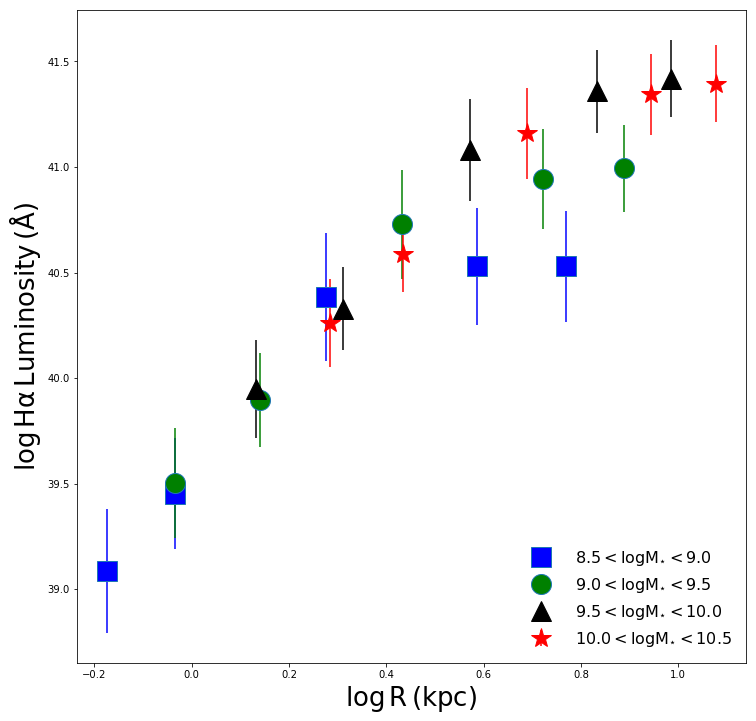
\includegraphics[width=1.5 \columnwidth]{gradients_HA.png}
	\caption{Average radial gradients in $H\alpha$ equivalent width in a total (left panel) and differential (right panel) sense. }
     \label{fig:grad_EW}

\end{figure*}
%%%%%%%%%%%%%%%%%%%%%%%%%%%%%%%%%%%%%%%%%%%%%%%%%%%%%%%%%%%%%% 

%%%%%%%%%%%%%%%%%%%%%%%%%%%%%%%%%%%%%%%%%%%%%%%%%%%%%%%%%%%%%%
\begin{figure*}
	\centering
	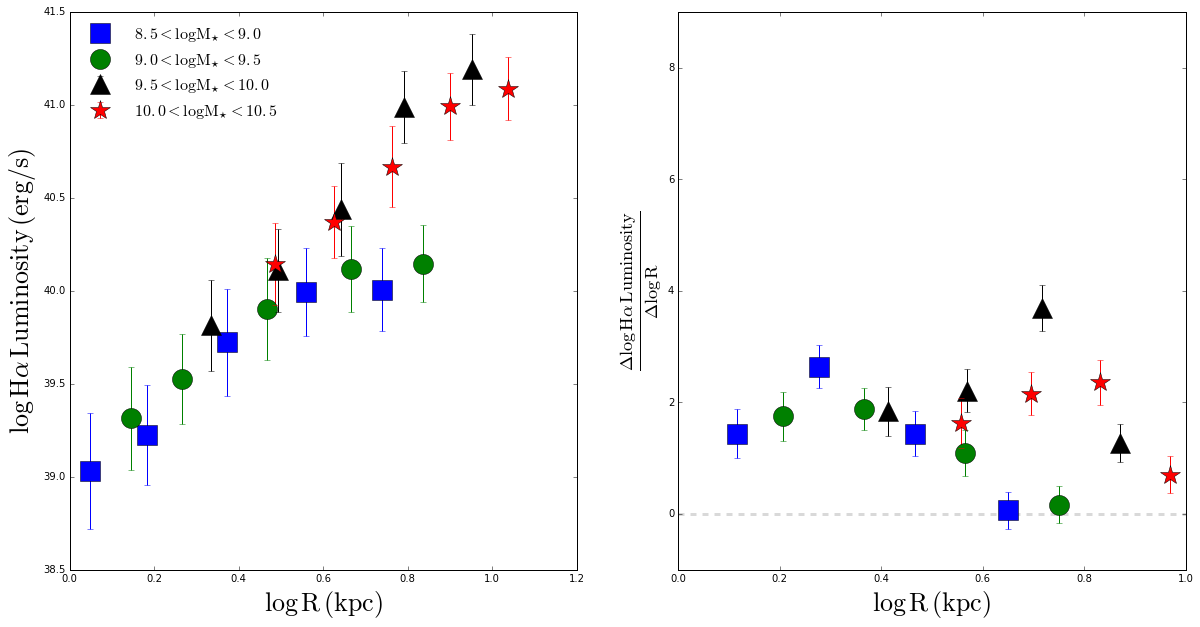
\includegraphics[width=1.5 \columnwidth]{gradients_HA_Lum.png}
	\caption{Average radial gradients in $H\alpha$ equivalent width in a total (left panel) and differential (right panel) sense. }
     \label{fig:grad_lum}

\end{figure*}
%%%%%%%%%%%%%%%%%%%%%%%%%%%%%%%%%%%%%%%%%%%%%%%%%%%%%%%%%%%%%% 

\section{Discussion}

\subsection{Radial Dependencies}

In Section \ref{sec:obs}, we describe our method for correcting spectroscopic measurements for regions of the galaxy that lie outside the SDSS fiber. To summarize, we define $\Psi$ as the fraction of the galaxy that lies within the fiber, and assume the correction factor is a power law in $\Psi$, with the power law index determined empirically. This power law index could be in principle a function of any number of galaxy parameters; here we subdivided our sample into four mass bins and determined the power law index for each bin.

Because we can correct for fiber effects we can use both the fiber measurement and the corrected measurement to probe the galaxy at two radii, the full effective radius and the fiber radius. This allows us to plot radial profiles for the parameters we are interested in, $H\alpha$ luminosity and $H\alpha$ equivalent width. Particularly striking is the profile of $H\alpha$ luminosity. In high mass galaxies, the profile is consistent with a single power law at all radii, whereas in galaxies below $10^{9.5} \rm M_{\odot}$ in stellar mass, the profile resembles a broken power law. The power law slope is consistent with the high mass slope at small radii, then at intermediate radii it flattens out, consistent with no $H\alpha$ emission at larger radii. Although we have limited spatial resolution, the transition radius occurs at $3-4$ kpc.

The presence of $H\alpha$ purely at the center of galaxies is significant evidence against in-situ star formation in the outskirts of dwarf galaxies. Although we are only looking at low-redshift dwarfs, detailed studies of local dwarfs' star formation histories show a wide range of formation times, suggesting that if dwarf galaxies formed stars in their outer regions at early times, we would expect to see extended star formation reflected in the radial profiles. This is not observed; however, it is possible that extended star formation in dwarf galaxies took place at an earlier stage in the Universe's history. Similar observations at higher redshift would rule out this possibility.

%%%%%%%%%%%%%%%%%%%%%%%%%%%%%%%%%%%%%%%%%%%%%%%%%%%%%%%%%%%%%%
\begin{figure*}
	\centering
	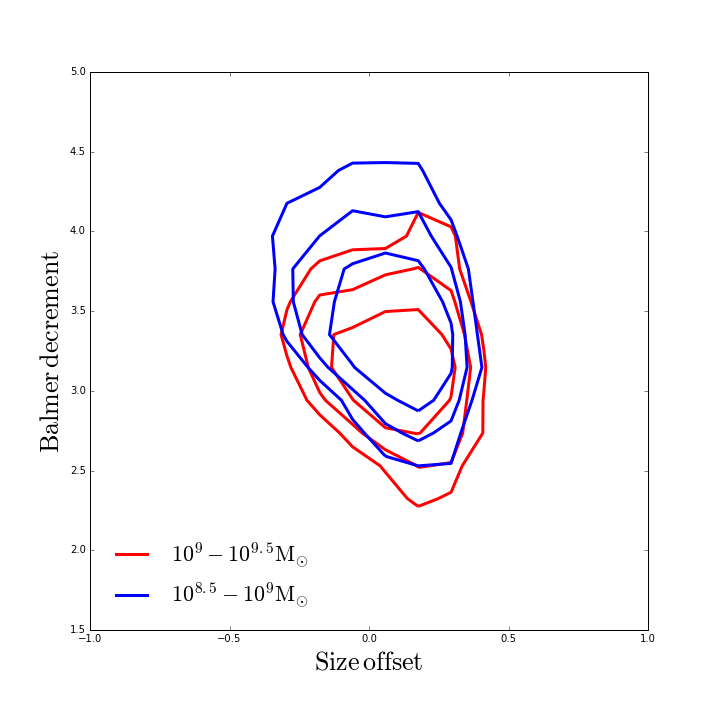
\includegraphics[width=1.5 \columnwidth]{BD_size.png}
	\caption{Balmer decrement vs. size offset for dwarf galaxies.}
     \label{fig:bdvsize}

\end{figure*}
%%%%%%%%%%%%%%%%%%%%%%%%%%%%%%%%%%%%%%%%%%%%%%%%%%%%%%%%%%%%%% 


\subsection{Galaxy Size}

An important prediction of the ``breathing'' model of feedback regulation in dwarf galaxies is that star formation rate is anticorrelated with galaxy size. In the model, stars are formed in the galactic center. The young stars then produce supernova feedback, which blows out the reservoir of gas from which the stars were formed, dampening star formation. As a result, galaxies are actively forming when they are at their smallest. During the subsequent blowout phase the galaxy will be more diffuse and, if the galactic wind drives radial transport, the galaxy will have a larger effective radius \cite{EB17}. 

Our results give compelling evidence for this prediction below $10^{9.5} M_{\odot}$, suggesting that dwarf galaxies form stars in a ``breathing" mode. Importantly, this result combined with the lack of $H\alpha$ seen in galactic outskirts of dwarfs suggests that the energy produced during episodes of star formation couples to the stars in the galactic center and drives stellar radial transport;  while this isn't direct evidence of feedback energy coupling to dark matter, evidence of collisionless stars being dredged out of the galactic interior is a strong indication that collisionless dark matter is transported as well well. This is significant, as this coupling of a dwarf galaxy's feedback to its dark matter halo is one method of dark matter heating that is often invoked in order to reconcile the cored profiles seen in dwarfs in the real Universe with the cuspy profiles predicted by $\Lambda$CDM. 

There are, however, alternate explanations for the observed anti-correlation between H$\alpha$ emission and galaxy size. Galaxies may be also producing stars at the same rates across different sizes and emitting different amounts of $H\alpha$ light. We will briefly discuss these.

The first explanation, that galaxies at different sizes do form stars at the same rate, but different amounts of $H\alpha$ emission escape the galaxy. This could be due to variations in the initial mass function (IMF), which sets the rates at which stars of different masses form. A top-heavy IMF, where more massive stars are formed relatively more frequently, would result in more ionizing radiation being formed per unit star formation, resulting in correspondingly more ionizing radiation per unit star formation. Our results could potentially be explained by smaller galaxies having more top-heavy IMFs. Whether or not the IMF varies between galaxies, or within galaxies, is an area of active research, with most results being consistent with a universal IMF \citep[e.g.,][]{Bastian10}. 

An alternate possibility is that galaxies form stars at the same rate and as described by the same IMF, but smaller galaxies have a higher escape fraction for $H\alpha$ radiation. We can test that possibility by testing whether the Balmer decrement is a function of galaxy size, shown in Figure \ref{fig:bdvsize}. Galaxies with small sizes tend to have higher Balmer decrements than those that have larger sizes. This implies that the escape fractions of Balmer series emission in larger galaxies is on average higher than it is in smaller galaxies; thus, differential escape fractions can not explain our results.

\subsection{Duty Cycle and Energetics}

In Section \ref{sec:results}, we calculate the duty cycle of the active phase of the dwarf galaxies to be approximately 1/3; i.e., dwarf galaxies spend roughly one third of their lifespan in their actively forming stars and the other 2/3 in their blowout phase. There are several different interpretations for this number that we will now go through.

Firstly, we will examine this number under the view that the instantaneous star formation rate in dwarf galaxies at a particular time is a stochastic sampling of an underlying probability distribution of star formation rates. Of course, this view is only sensible as an approximation; nevertheless, there are benefits to thinking of star formation in this way, particularly as it pertains to generating analytic and semi-analytic models \citep{Kelson16}. 

Under this probabilistic interpretation, a galaxy's star formation rate represents a sampling of an underlying star formation rate probability distribution function. Our result suggest that the probability of galaxies being in the quiescent state is twice as high as the galaxies in the active state. We draw a distinction between this quiescent phase and final quenching, when a galaxy becomes ``red and dead." This final quenching phase is likely not a result of stochastic sampling of an underlying pdf, but rather the result of physical processes that bring the galaxy out of the ``breathing'' mode and into the ``red and dead'' mode. In particular, galaxies at these masses are predominantly quenched through environmental means \citep{geha12}.

Physically, we can interpret duty cycle in terms of the times the galaxy spends in each phase in order to explore the physicals scalings and energetics involved. As an example, we use the test case of a $10^9 M_{\odot}$ galaxy of radius 5 kpc. Assuming that the blowout moves with the speed $v_{wind}$, the total time it takes to reach the edge of the galaxy is $\frac{R}{v_{wind}}$. If the material takes the same amount of time to fall back onto the center as to reach the galactic outskirts, then we can conclude empirically that the time spent in the active phase during a single burst is $$t_{active} = \frac{R}{v_{wind}} = 16.3 Myr \times \frac{R}{5 kpc}\times \frac{300 km/s}{v_{wind}}  $$, consistent with the timescales put forward by \cite{EB17}. Multiplying this value by the star formation rate of objects in the active phase gives us the total number of stars formed in one cycle:
$$\Delta M_{\star} = 1 \times 10^6 M_{\odot} \times \frac{SFR}{0.062 M_{\odot}/yr} \times \frac{t_{active}}{16.3 Myr}$$.

The IMF allows us to connect the amount of star formation in a burst to the amount of supernova feedback produced by that burst. Under a Kroupa IMF \citep{Kroupa02}, we expect one Type II supernova for every 100 solar masses in stars formed, meaning that a single burst in a dwarf galaxy produces some $10^4$ Type II supernova. Given that the average energy output of a Type II supernova is $10^{51}$ erg, the total energy output during a single burst is $10^{55}$ erg. In order to produce $10^9 M_{\odot}$ of solar mass, the galaxy must have gone through $10^3$ cycles, thereby producing $10^{55}$ erg of supernova energy in the process. The energetic argument presented in the above paragraph is true independent of whether the stars are formed constantly or in bursts. However, as several authors \citep{Governato12,GK13} have argued, the ``bursty'' mode of star formation can produce a positive feedback cycle, where the the efficiency of subsequent bursts increases from the initial burst. This also explains why more massive galaxies have cuspy profiles despite producing more supernova feedback; their star formation histories are less bursty \citep{Guo16}, so the feedback which drives us the average efficiency is not present.

\subsection{Comparisons to Simulations}

Hydrodynamical simulations whereby galaxy growth is regulated through burst-driven radial transport make a number of specific, testable predictions of galaxy observables. We divide our discussion of these predictions into two sections: predictions concerning galaxy dynamics, which primarily concerns the work of \cite{Cicone16}, and predictions concerning galaxy structure, which primarily concerns this work.

The burst-driven transport model of galaxy self-regulation requires that feedback not just couple to the gas in a galaxy, but also to the stellar component. As a result, the stars are kinematically heated, resulting in an increased line of sight velocity dispersion. \cite{El-Badry17} makes this prediction explicit, demonstrating a correlation between $\sigma_{LOS}$ and specific star formation rate for star particles in the final 40 snapshots of one dwarf galaxy halo. Under the assumption that the evolution of this single halo is an ergodic process, this supplies a prediction for the population of dwarf galaxies at low redshift.

These predictions are borne out by the analysis of \cite{Cicone16}, which uses stacked SDSS spectra to examine the profiles of nebular emission lines and stellar absorption lines, constraining the dynamics of galactic gas and stars respectively. They finds that, for dwarf galaxies, the width of stellar absorption lines increases with increasing specific star formation rate, consistent with the predictions of \cite{El-Badry17}. Furthermore, they find that this trend disappears above stellar masses of $32wee010^{9.5} M_{\odot}$, consistent with the prediction that burst-driven transport only operates at dwarf mass scales.

We can also compare the trends with size that we have explored in this work to predictions from hydrodynamical simulations. In Figure \ref{fig:predict}, we overplot the final 40 snapshots from a dwarf galaxy in the fire simulation with galaxies from our lowest-mass bin ($10^{8.5}-10^{9.0} M_{\odot}$) in specific star formation rate/size space. Again, we emphasize that since the simulated galaxies evolve in this space, the points traced by the galaxy in the simulation make a prediction for galaxies sampled in the real Universe. We see excellent agreement between the predictions made by the simulation and our observed relationship between specific star formation rate and size. There is significantly more scatter in the observed relation than the simulation results, which is a natural result of comparing an ensemble of galaxies with a single simulated object, but the overall agreement between simulations and data is striking. Taken together, these two observational confirmations of simulation predictions provide strong evidence that burst-driven radial transport is occuring in dwarf galaxies.



%%%%%%%%%%%%%%%%%%%%%%%%%%%%%%%%%%%%%%%%%%%%%%%%%%%%%%%%%%%%%%
\begin{figure*}
	\centering
	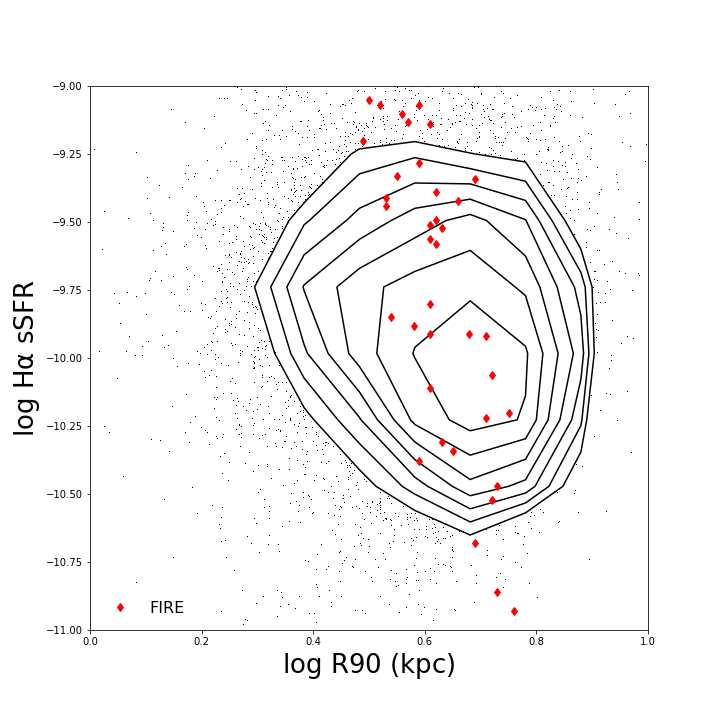
\includegraphics[width=1.5 \columnwidth]{111_dwarf_85_size_SF_r.png}
	\caption{Star formation rate plotted against size for galaxies in our lowest mass bin. Overplotted are points from the last 40 snapshots of a dwarf galaxy in the FIRE simulation that is undergoing self-regulation via burst-driven radial transport. The data is in excellent agreement with the predictions from the simulations}
	\label{fig:predict}
	
\end{figure*}
%%%%%%%%%%%%%%%%%%%%%%%%%%%%%%%%%%%%%%%%%%%%%%%%%%%%%%%%%%%%%% 

\section{Conclusion}

Our study primarily examines the relationship between the physical size of a galaxy and it's star formation properties. We show the following,

\begin{itemize}
\item Dwarf galaxies with smaller size tend to have higher levels of $H\alpha$ emission. Larger galaxies have lower levels of $H\alpha$ emission. This trend goes away in more massive galaxies. 

\item $H\alpha$ surface density is consistent with a power law with respect to radii in the inner regions of all galaxies at all masses, however in dwarf galaxies, the outer regions have $H\alpha$ emission consistent with zero.

\item Taken together, these results paint a picture of dwarf galaxies experience cycles of star formation, where dense star formation in the central regions drives blowouts that self-regulate galaxy growth. Furthermore, our results are in strong agreement with simulations that exhibit such blowouts. The energy of the blowouts couples to the stars, leading to dwarf galaxies in their blowout phase being larger on the sky in the $r$ band. This apparent coupling to stars, and not just gas, could indicate coupling to dark matter as well.

\end{itemize}

\bibliographystyle{ApJ}
\bibliography{biblio}

\appendix{Comparison to color-based aperture corrections}

Here we compare our aperture correction method to one similar to that of \cite{Brinchmann04}. In order to correct for the size of the SDSS fiber, the authors developed a methodology whereby a spectroscopic measurement (e.g. star formation rate) was associated with the fiber $gri$ colors of the galaxy, the the properties of the galaxy outside of the fiber were inferred from the gri colors of the portion of the galaxy located outside of the fiber. Here, we adopt a similar methodology for the purposes of comparison. 

%%We adopt a simple, yet effective relation to estimate $H\alpha$ equivalent width from galaxy color:

%%$$\rm log EW_{H\alpha} = 2-%%2\times(\textit{g-r}) $$

%%

We first make use of the fiber g-r and r-i colors to estimate to estimate the measured fiber equivalent width. We divide the sample in half, and use the two colors as features in decision-tree regression algorithm fit to fiber $H\alpha$ equivalent widths. We then use the algorithm to predict the fiber $H\alpha$ equivalent width in the unused half of the sample. The agreement between the prediction derived from the colors and the spectroscopic measurement is seen in Figure \ref{fig:ccheck}. Then, we estimate the total $H\alpha$ equivalent width from the galaxies' total colors. The red contours in Figure \ref{fig:ccheck} demonstrate the agreement between the equivalent width estimated in this way and the equivalent width determined from the fiber corrections described in \ref{sec:fibercor}.

Below $10^{9.5}$ solar masses, we see the agreement between the two methodologies break down. Predictions of total galaxy $H\alpha$ equivalent widths based on fiber color will tend to be overestimates, particularly in low equivalent width systems. This observation  in line with what \cite{Salim07} argued; the relation between color and SSFR established in star forming galaxies breaks down in galaxies without $H\alpha$. We point out that this also extends to regions of galaxies that do not emit $H\alpha$, which impacts fiber corrections even within star forming galaxies.

%%%%%%%%%%%%%%%%%%%%%%%%%%%%%%%%%%%%%%%%%%%%%%%%%%%%%%%%%%%%%%
\begin{figure*}
	\centering
	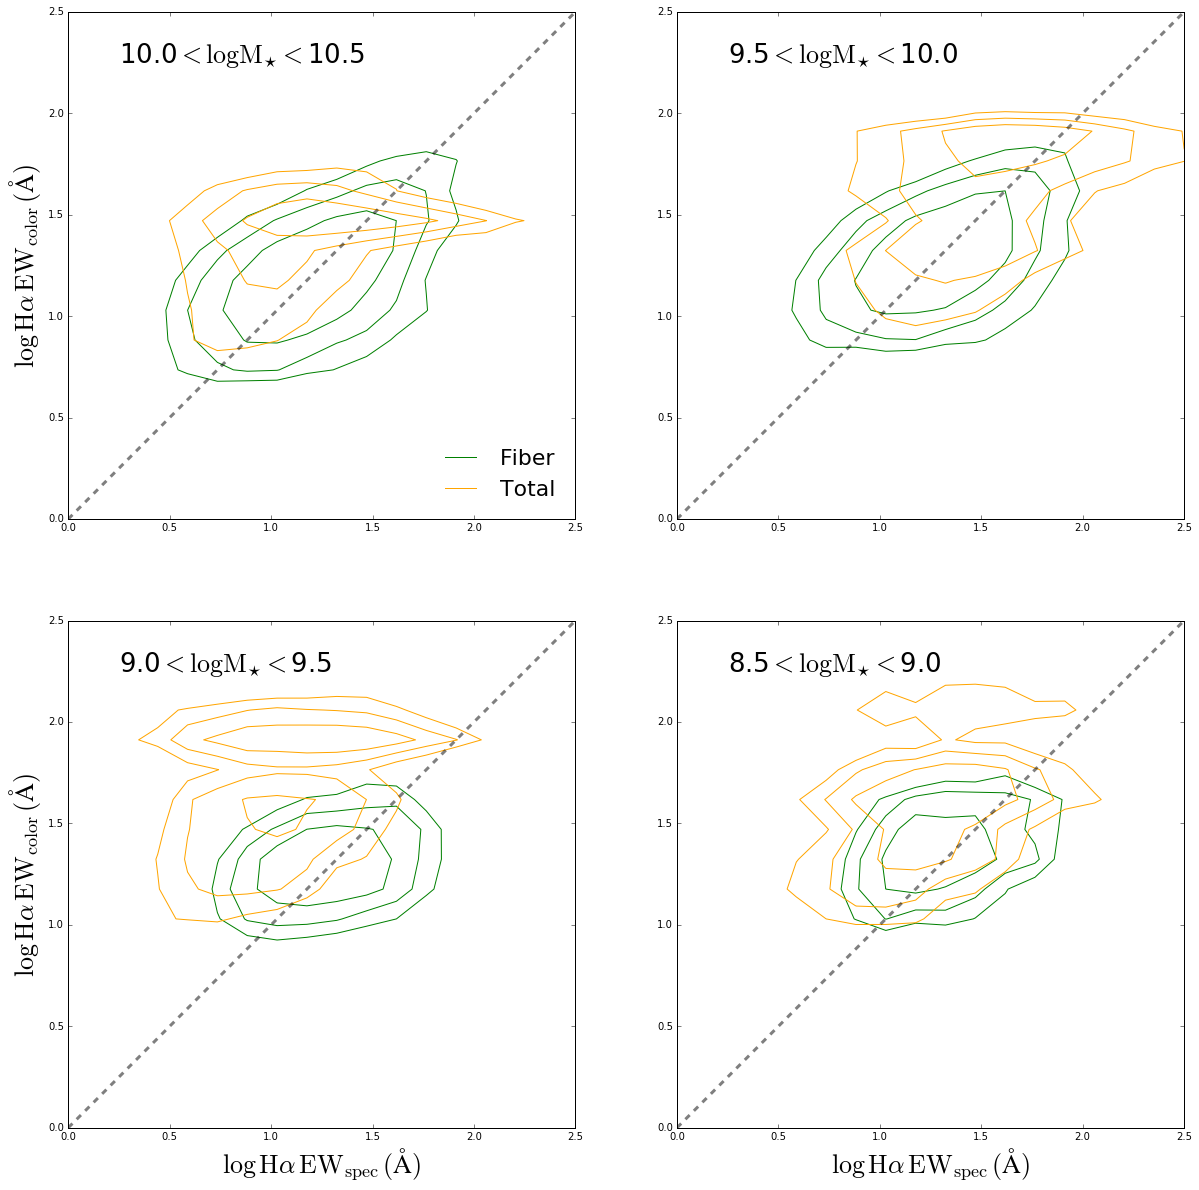
\includegraphics[width= \columnwidth]{HA_EW_compare.png}
	\caption{Comparison between photometrically-derived and spectroscopically-derived $\rm H\alpha$ equivalent widths for galaxies in our science sample (see text for details). Blue contours are the $H\alpha$ within the fiber and red contours are total $H\alpha$. At low masses, the photometrically derived total $H\alpha$ is overestimated.}
     \label{fig:ccheck}

\end{figure*}
%%%%%%%%%%%%%%%%%%%%%%%%%%%%%%%%%%%%%%%%%%%%%%%%%%%%%%%%%%%%%% 

\end{document}

%%
%% End of file `sample.tex'.
